\documentclass[conf]{new-aiaa}
%\documentclass[journal]{new-aiaa} for journal papers
\usepackage[utf8]{inputenc}

\usepackage{graphicx}
\usepackage{amsmath}
\usepackage[version=4]{mhchem}
\usepackage{siunitx}
\usepackage{longtable,tabularx}
\usepackage{footnote}
\usepackage{mhchem}
\usepackage{physics}
\usepackage{array,makecell,booktabs}
\newcolumntype{M}[1]{>{\centering\arraybackslash}m{#1}}
\usepackage[super]{nth}
\makesavenoteenv{tabular}
\setlength\LTleft{0pt}

\graphicspath{{figures/}}

\begin{document}

\section{Discussion}

This section presents estimates of the cost-per-flight of various reuse strategies. Two strategies, (downrange, rocket-propelled, propulsive landing, full recovery) and (downrange, no propulsion, parachute, full recovery), are shown to dominate the other strategies on cost. However, parachute recovery of the full first stage is likely only practical for small launch vehicles\footnote{A small stage on parachutes could be recovered in midair or on a ship, or survive landing on land. A large stage on parachutes may need to land directly in the ocean, which would increase recovery and refurbishment expenses.}, and it will also be shown that first stage reuse is not favorable for small launch vehicles. Thus, downrange propulsive landing appears to be the dominant strategy.

Launch rate is also a critical factor in the economics of reuse. Increasing launch rate further reduces cost-per-flight, and also allows the investment in reuse development to be paid off more quickly. Efficient first stage reuse may allow for an increase in launch rate. A market that can support a high (>20 flights/year) launch rate may be a critical factor for the economic viability of a first stage reuse.

The discussion is organized as follows: the first subsection shows the distribution of cost-per-flight estimates under a generic dispersion of the model input parameters. The subsequent subsections examine the effect of number of reuses, launch rate, and launch vehicle size on cost. Finally, the last section discusses whether the present value of cost savings from reuse is enough to justify the initial investment in its development.

\subsection{Strategy Cost-per-flight Estimates}
violin plots of strategy cpfs
cpf varies with technology choice, mission, large uncertainties with winged vehicles

\subsection{Effect of Number of Reuses and Launch Rate}
stack plot with reuse sweep- show why cost declines with number of reuses
cpf vs. reuse plot with varying launch rate curves - shows significant decrease in cost with increasing launch rate for low launch rates
cpf vs. reuse plot for different strategies 

In order to look at the breakdown of costs for a launch vehicle with a reusable first stage, we consider a point cost estimate to demonstrate general trends. The following example evaluates a two stage launch vehicle carrying a 10,000 kg payload to LEO using kerosene and liquid oxygen propellants at a launch rate of 15 launches per year. We consider the case of a propulsive downrange landing to recover and reuse the entire first stage. The cost per flight is determined over a range of number of first stage uses. The results of this analysis are shown in Figure \ref{fig:cpf_stackplot_reuses_sweep}.

\begin{figure}[hbt!]
    \centering
    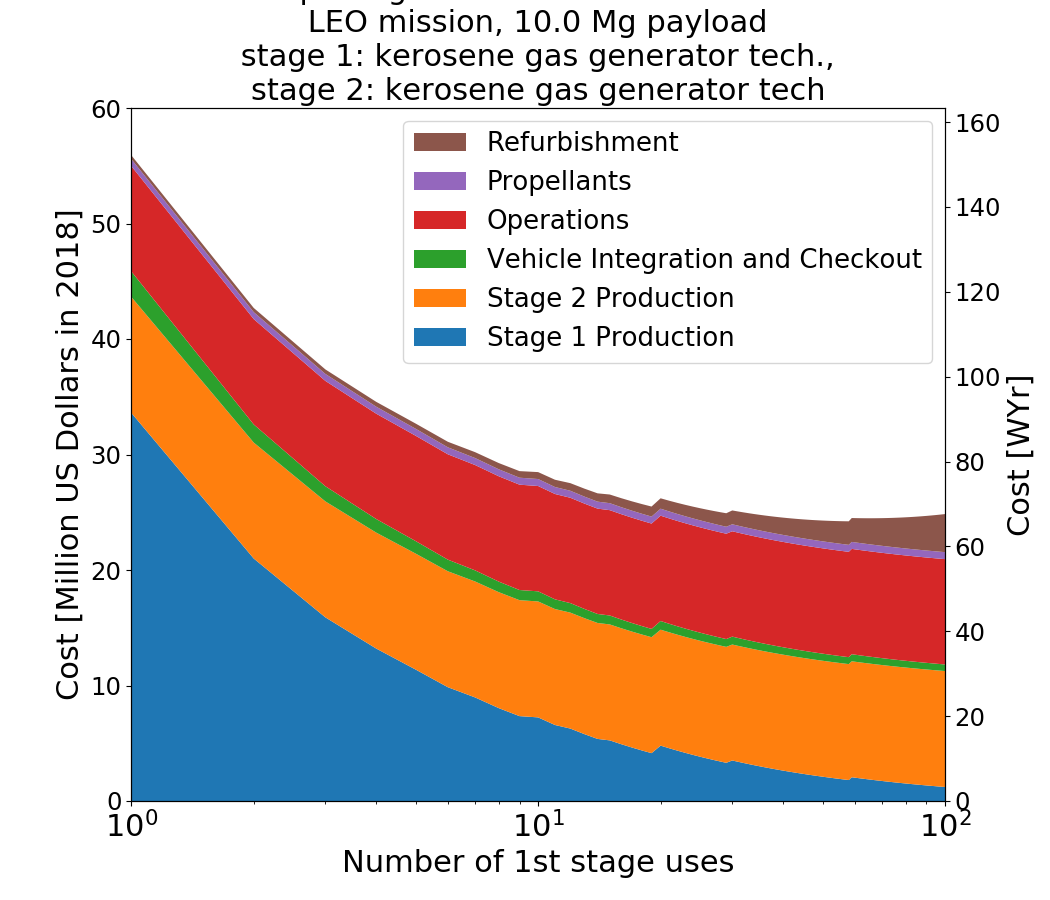
\includegraphics[width=\textwidth]{../../lvreuse/analysis/combined/plots/cpf_stackplot_reuses_sweep}
    \caption{\label{fig:cpf_stackplot_reuses_sweep} TODO caption.}
\end{figure}

Several things should be noticed from the results in Figure \ref{fig:cpf_stackplot_reuses_sweep}. First, the stage one productions costs per flight decrease dramatically as we increase the number of first stage reuses. This result is very intuitive -- as the cost of first stage production is spread over a larger number of flights, the per flight amortization share of the first stage production cost decreases. This leads to a reduction in the cost per flight. However, this trend of decreasing amortization share of first stage production costs is opposed by the refurbishment cost trends. As the number of first stage uses increases, the refurbishment cost per flight also increases. This is due to the fact that more components on the first stage will need inspected or replaced  as the number of reuses increases. 

These opposing trends lead to an interesting result: the total cost per flight trend achieves a minimum value. In the example in Figure \ref{fig:cpf_stackplot_reuses_sweep}, we see a minimum cost per flight around 57 first stage uses. After 57 uses of the first stage, it would be more cost effective to use a new first stage than to continue refurbishing the old one. 

\begin{figure}[hbt!]
    \centering
    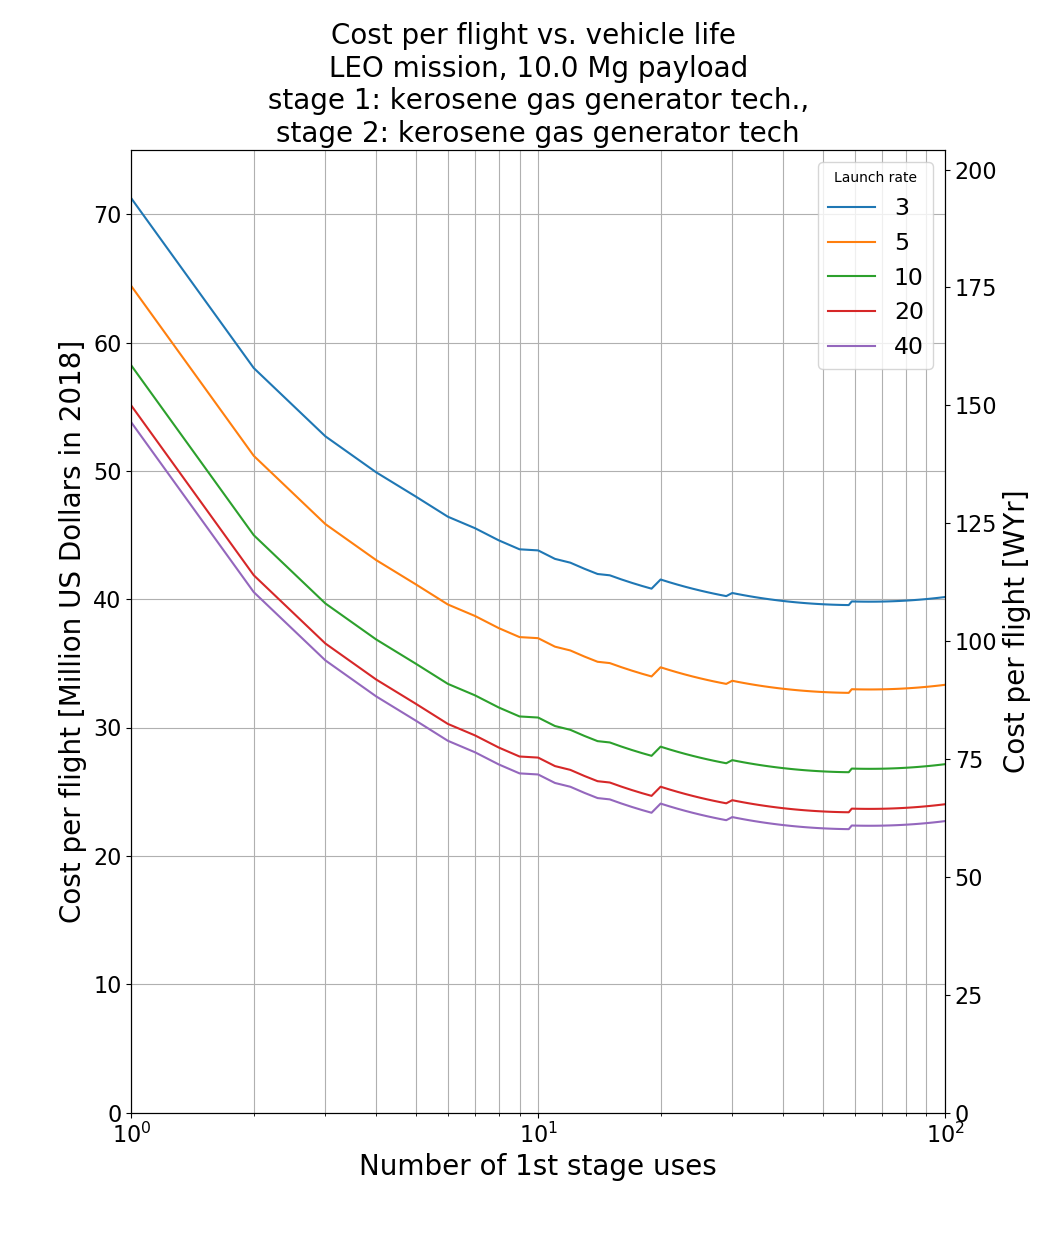
\includegraphics[width=\textwidth]{../../lvreuse/analysis/combined/plots/cpf_reuses_sweep_vary_launch_rate}
    \caption{\label{fig:cpf_reuses_sweep_vary_launch_rate} TODO caption.}
\end{figure}

\subsection{Effect of Launch Vehicle Size}
reuse doesn't make sense for smaller vehicles - costs not dominated by hardware cost

\subsection{Paying off development costs}
npv plot

\bibliography{first_stage_recovery}

\end{document}